%==============================================================================
%  Movie Recommendation Hub -- PSIA 2026/2027 Project Report
%  Group 17 -- Instituto Superior Tecnico, Universidade de Lisboa
%  ACM-like two-column look, adapted to the PSIA rules:
%  Times 10pt, 2.0 cm side margins, 1.5 cm top/bottom, single spacing, <= 5 pages.
%  Compile: latexmk -pdf -jobname=project-g17 main.tex
%==============================================================================
\documentclass[10pt,a4paper,twocolumn]{article}
\usepackage[T1]{fontenc}
\usepackage[utf8]{inputenc}
\usepackage{mathptmx}                 % Times New Roman
\usepackage[scaled=0.92]{helvet}      % ACM-like sans headings
% The page numbers sit 1.6 cm from the bottom, so all of them stays clear of the 1.5 cm margin. The text
% ends where it would with bottom=1.5cm and footskip=0.6cm.
\usepackage[left=2.0cm,right=2.0cm,top=1.5cm,bottom=1.6cm,columnsep=0.6cm,includefoot,footskip=0.5cm]{geometry}
\usepackage{graphicx,booktabs,tabularx,enumitem,xcolor,amsmath}
\usepackage[hidelinks]{hyperref}
\usepackage{titlesec}
\usepackage[font=small,labelfont=bf,skip=3pt]{caption}

% ---- ACM-style headings ------------------------------------------------------
\titleformat{\section}{\sffamily\bfseries\normalsize\MakeUppercase}{\thesection}{0.6em}{}
\titleformat{\subsection}{\sffamily\bfseries\normalsize}{\thesubsection}{0.6em}{}
\titleformat{\subsubsection}[runin]{\itshape}{}{0em}{}[.]
\titlespacing*{\section}{0pt}{6pt}{3pt}
\titlespacing*{\subsection}{0pt}{4pt}{2pt}
\titlespacing*{\subsubsection}{0pt}{2pt}{0.5em}
\setlist{leftmargin=1.1em,nosep}
\setlength{\parskip}{0pt}
\setlength{\textfloatsep}{6pt plus 2pt}
\setlength{\floatsep}{6pt plus 2pt}
\setlength{\abovecaptionskip}{3pt}

% ---- Placeholders for work still to be done ----------------------------------
% \TODO{...}  : short red inline placeholder (to replace once implemented)
% \PH{...}    : a whole placeholder paragraph, boxed in red
\newcommand{\TODO}[1]{\textcolor{red}{\textbf{[TODO:} #1\textbf{]}}}
\newcommand{\PH}[1]{\par\noindent\fcolorbox{red}{red!4}{\parbox{\dimexpr\linewidth-2\fboxsep-2\fboxrule}{\small\textcolor{red!70!black}{\textbf{PLACEHOLDER.} #1}}}\par}
\newcommand{\code}[1]{\texttt{#1}}

\begin{document}

% ---- Title block (ACM-like) --------------------------------------------------
\twocolumn[{%
\begin{center}
{\sffamily\bfseries\LARGE Movie Recommendation Hub: An AI-Powered,\\[2pt] Microservices-Based Platform on Self-Hosted Kubernetes\par}
\vspace{6pt}
{\sffamily\small PSIA 2026/2027 -- Project Report -- \textbf{Group 17}\par}
\vspace{6pt}
\begin{tabular}{ccc}
{\sffamily Manuel Fernandes} & {\sffamily Jo\~ao Russo} & {\sffamily Tiago Fonseca}\\
{\small 106410} & {\small 116543} & {\small 112346}\\
\end{tabular}\\[2pt]
{\small Instituto Superior T\'ecnico, Universidade de Lisboa, Lisbon, Portugal}\\[4pt]
{\small \textbf{Video:} \url{https://youtu.be/Drgl3k404wE} \;\textbar\; \textbf{Repository:} \url{https://gitlab.rnl.tecnico.ulisboa.pt/psia/groups26/g17}}
\end{center}
\vspace{4pt}
}]

% 01-introduction
\section{Introduction}\label{sec:intro}

The goal of the PSIA project is to deploy a realistic, tiered, microservices-based application with AI components on a public cloud, using Infrastructure-as-Code (IaC) end to end: virtual machines are provisioned with Terraform, configured with Ansible, and orchestrated by a \emph{self-hosted} Kubernetes cluster (managed offerings such as GKE are not allowed). The system must also be instrumented and observed with a monitoring stack, and extended with one advanced feature.

Our application is a \emph{Movie Recommendation Hub}. Users register and log in through Keycloak (OpenID Connect~\cite{oidc}), keep a profile with their favourite genres, watched movies and the users they follow, browse and search a catalogue of about 45\,000 movies from The Movies Dataset~\cite{banik2017movies}, and view other users' profiles to discover new interests. An AI inference engine, a small open language model (Qwen2.5~3B) served by Ollama on the VMs' CPUs, together with a sentence-embedding model (\code{nomic-embed-text}) for search by meaning, produces personalised recommendations in two ways: \emph{on demand}, when a user asks for suggestions, optionally with free-text constraints (``a horror movie from the 80s''); and \emph{proactively}, through a background agent that precomputes and caches recommendations per profile, so that users are greeted with fresh suggestions as soon as they log in. Following the database-per-service pattern~\cite{richardson-dbps}, each backend service owns its own PostgreSQL database.

The system runs on Google Cloud Platform (region \code{europe-west4}), on a kubeadm cluster of three VMs (one control-plane node and two workers), and is monitored with Prometheus~\cite{prometheus} and Grafana. As advanced feature we chose \emph{persistent state}: every VM of the deployment can be shut down and restarted without losing any application state.

The rest of this report is organised as follows. Section~\ref{sec:design} presents the architecture, services, data and deployment pipeline. Section~\ref{sec:advanced} describes the persistent-state design and its validation. Section~\ref{sec:eval} studies throughput and latency as the number of concurrent clients grows, and Section~\ref{sec:conclusion} concludes. The demonstration video is available at \url{https://youtu.be/TODO}, and the source code and deployment instructions are in the group repository at \url{https://gitlab.rnl.tecnico.ulisboa.pt/psia/groups26/g17}.

\section{System Design and Architecture}\label{sec:design}
% 02a-overview -- follows \section{System Design and Architecture}
The system follows the tiered microservices architecture of the specification (Fig.~\ref{fig:architecture}). The \emph{frontend tier} is a Next.js web application, the only entry point exposed to users; in the cluster it sits behind an NGINX reverse proxy that terminates TLS and routes \code{/} to the frontend, \code{/api/*} to the services, \code{/auth/} to Keycloak and \code{/grafana/} to Grafana. Users register and log in through \emph{Keycloak}, an OpenID Connect (OIDC) identity provider: the browser obtains a short-lived (5\,min) JWT access token and sends it as a \code{Bearer} header to every API call. The \emph{backend tier} consists of four Quarkus services: the \emph{Movies API} (catalogue browsing, full-text search and search by meaning), the \emph{Profiles API} (favourite genres, watched and saved movies, follow graph), the \emph{Recommendation API}, which stores recommendations and queues the work, and the \emph{recommendation worker}, which consumes that work from \emph{Apache Kafka} and queries the \emph{inference engine}, Ollama. Each API validates the token's signature, issuer and its own audience (\code{movies-service}, \code{profiles-service}, \code{recommendation-service}), so tokens minted for other clients are rejected; the recommendation service and the worker call the other services with their own Keycloak service-account tokens. The \emph{data tier} is PostgreSQL~16, with one instance per service (movies, profiles, recommendations) and one for Keycloak; each is migrated by Flyway, and services read each other's data only through their APIs. A \emph{monitoring server} (Prometheus, Grafana) scrapes all components. Table~\ref{tab:components} summarises the components and their status.

\begin{table}[t]\centering\footnotesize

\caption{System components and implementation status.}\label{tab:components}
\begin{tabularx}{\columnwidth}{@{}l>{\raggedright\arraybackslash}X l@{}}
\toprule
\textbf{Component} & \textbf{Technology} & \textbf{Status}\\
\midrule
Frontend & Next.js 16, React 19, Tailwind 4, keycloak-js & Done\\
Identity provider & Keycloak 26 (OIDC, PKCE) & Done\\
Movies API & Quarkus 3.39, Hibernate Panache, Flyway, pgvector & Done\\
Profiles API & Quarkus 3.39, Hibernate Panache, Flyway & Done\\
Recommendation API + agent & Quarkus, Kafka, background agent & Done\\
Recommendation worker & Quarkus, Kafka consumer & Done\\
Inference engine & Ollama (CPU), Qwen2.5~3B, nomic-embed-text & Done\\
Message queue & Apache Kafka 4.3 (Strimzi, 3 brokers) & Done\\
Databases & PostgreSQL 16, one instance per service & Done\\
Container images & Multi-stage Dockerfiles (backend, frontend) & Done\\
Local deployment & Docker Compose (infra, backend, frontend), \code{just} & Done\\
Cluster (IaC) & Terraform, Ansible, kubeadm on GCP & Done\\
Reverse proxy & NGINX with TLS & Done\\
Monitoring & Prometheus, Grafana, Micrometer & Done\\
Persistent state (advanced) & StatefulSets, local-path volumes & Partial\\
\bottomrule
\end{tabularx}
\end{table}

\begin{figure*}[t]\centering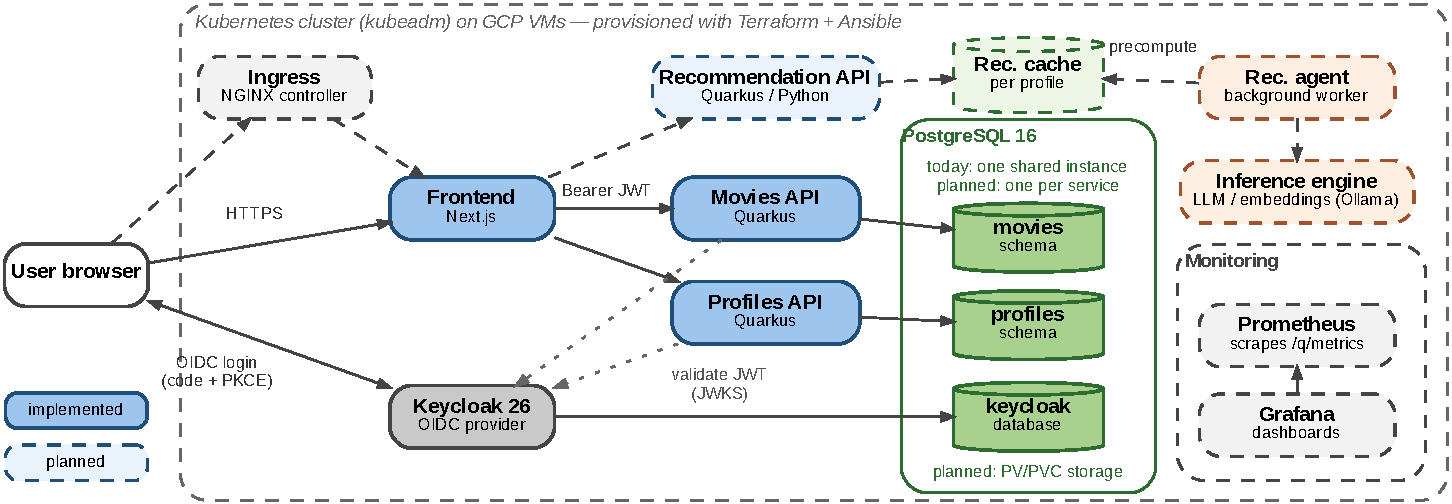
\includegraphics[width=\textwidth]{figures/architecture.pdf}\caption{Architecture of the Movie Recommendation Hub. Colours: blue = application services, green = data, orange = AI, grey = infrastructure/operations (dotted arrows are JWT validation). All components shown are now implemented: four Quarkus services, one PostgreSQL instance per service, Kafka between the recommendation service and its worker, Ollama as inference engine, and an NGINX reverse proxy in front of a self-hosted Kubernetes cluster. \TODO{regenerate this figure (\code{figures/architecture\_gen.py}, rendered with \code{neato}): it still draws the planned components with dashed outlines and omits Kafka and the worker.}}\label{fig:architecture}\end{figure*}

% 02b-backend
\subsection{Backend Services, Data and AI}

Each service is a Quarkus application whose schema Flyway owns. The catalogue comes from The Movies Dataset, whose \code{movies\_metadata.csv} was cleaned (column-shifted rows and duplicate ids dropped, genre lists parsed) into 45\,430 movies and 20 genres, shipped as a \code{pg\_dump}. Profiles store only movie and genre ids, with no foreign keys across databases, so the Profiles API checks ids through the Movies API before storing them. A profile is created on the user's first authenticated request, from the token's subject and username.

\subsubsection{Search} \code{GET /movies/search} uses PostgreSQL full-text search over weighted, accent-insensitive title and description vectors, prefix matching on title words, and a trigram fallback for typos, ranked in four tiers (title match, title prefix, description, similar title). For \emph{Ask AI}, the Movies API also searches \emph{by meaning}. A background job stores a 768-dimensional \code{nomic-embed-text} vector for each of the $\sim$9\,100 movies with at least 50 votes in pgvector, and a request is ranked by vector similarity.

\subsubsection{Recommendations} A set of ten recommendations takes the model minutes on a CPU, so the work is asynchronous. The Recommendation API answers at once (\code{202}) and puts a job, with a snapshot of the profile, on the Kafka topic \code{recommendation.requests} (6 partitions, keyed by user). The worker takes one job at a time and publishes the result on \code{recommendation.results}. The API stores it, and a third topic, \code{recommendation.ready}, lets every API instance notify its connected browsers through server-sent events. A job leaves the queue only once it is done, so a worker that stops mid-job leaves it for the next one. There are two kinds of request, \emph{Recommended for you}, made from the profile and what followed users watched, and \emph{Ask AI}, made from free text. The worker narrows the 45\,000 movies first. It turns the request into filters (genres, years, keywords), the Movies API returns 30 candidates (closest in meaning, then best rated) and up to 20 come from followed users, and the model chooses ten. Its answer must follow a JSON schema that only allows the candidates' ids, so it cannot invent movies, and if it chooses fewer than ten, the best-ranked candidates fill the gaps.

A \emph{background agent} runs every 10 minutes and keeps \emph{Recommended for you} current without redoing work. Each set records a fingerprint of the inputs it was made from, and the agent queues a new set only for profiles whose inputs changed (after 2 quiet minutes), at most 20 per run, retrying failures with exponential back-off. Identical inputs share results, and a request still pending after an hour is failed by a sweeper as a safety net.

\subsubsection{Model choice} We chose Qwen2.5~3B~\cite{qwen25} in Ollama because it fits the workers' memory with room for the rest of the system (about 2.5\,GB), runs on their CPUs, and follows Ollama's JSON-schema output, which our pipeline relies on to keep answers inside the candidate list. Smaller variants (0.5B, 1.5B) answer faster but choose less well, and a larger model would make each recommendation slower still on these CPUs. Narrowing the catalogue to 50 candidates before the model sees it keeps the prompt near 2\,000 tokens, which is what makes a 3B model usable. \code{nomic-embed-text}~\cite{nomic-embed} is a small embedding model (about 270\,MB) that the same Ollama server runs.

\subsubsection{Security and testing} Keycloak hosts a \code{movies} realm, imported from JSON, with self-registration, brute-force protection and two public clients (the frontend and the Swagger UIs). Each API exposes health checks, Prometheus metrics and OpenAPI. Tests run against a throwaway PostgreSQL through Quarkus Dev Services, with injected identities instead of Keycloak and in-memory channels instead of Kafka, while the worker's tests replace the model with a mock.

\subsection{Frontend}\label{sec:frontend}
The web interface is a Next.js~16 application in TypeScript. Its pages render in the browser and call the APIs directly. The pages are \code{/movies} (catalogue with search, sorting and infinite scrolling, topped by \emph{Recommended for you}), \code{/movies/[id]} (details, mark as watched, watch later), \code{/recommendations} (\emph{Ask AI} and the last five answers), \code{/users} and \code{/users/[id]} (profiles, follows). An \code{AuthGate} logs users in with \code{keycloak-js}, keeps the token only in memory and refreshes it before each call. Because recommendations take minutes, the interface never waits for them, and a fetch-based server-sent-events stream to the Recommendation API notifies the user when a result is ready. In the cluster the image uses relative addresses (\code{/api}, \code{/auth}), so one image works at any address.

\subsection{Deployment and Operations}\label{sec:deployment}
\subsubsection{Local deployment} The whole system runs locally in Docker, as three Compose projects that share one network (\code{movies-net}): \code{infra/compose.yaml} (databases, Kafka, Ollama, Keycloak), \code{backend/compose.yaml} (the four Quarkus services) and \code{frontend/compose.yaml} (the website). The infrastructure project runs three PostgreSQL~16 containers (the movies one with the pgvector extension), a single-broker Kafka in KRaft mode, Ollama with a one-shot container that downloads the two models, and Keycloak~26 (\code{start-dev --import-realm}), which imports the \code{movies} realm from \code{movies-realm.json} and keeps its state in its own database in the movies server. The movies container mounts \code{infra/init/}, whose script creates the \code{keycloak} role and database on first start. Every container has a health check (\code{pg\_isready}, Kafka's broker API, Ollama's \code{list}, the \code{/health/ready} endpoints). Because \code{depends\_on} cannot cross projects, a \code{justfile} starts them in order and waits for each to report healthy (\code{--wait}): \code{just local-first-up} also imports the \code{pg\_dump} catalogue before the backend starts, and \code{just local-up} skips the import. In containers the services run in Quarkus' production profile and read their database URLs, OIDC issuer and CORS origins from environment variables; Keycloak keeps the browser-facing address as the token issuer, while the services reach it by container name through its backchannel hostname setting.

\subsubsection{Containerization} A single multi-stage \code{backend/Dockerfile} builds any of the four Quarkus services from source (Maven in the build stage, a UBI9 OpenJDK~21 runtime in the final one), and \code{frontend/Dockerfile} builds the Next.js standalone server. The same Dockerfiles serve Compose and the cloud deployment, where \code{build-images.sh} builds the five images for \code{linux/amd64} and pushes them to Docker Hub.

\subsubsection{Kubernetes on GCP} The production target is a self-hosted cluster (managed offerings such as GKE are excluded by the specification), created entirely through IaC and driven from a management container that holds Terraform, Ansible, \code{kubectl} and \code{gcloud}. Terraform creates, in a separate stack that outlives the VMs, one data disk per worker and a reserved static IP, then a VPC and subnet, firewall rules and three Compute Engine VMs in \code{europe-west4-b} running Ubuntu 24.04: one control-plane node (\code{e2-standard-2}) and two workers (\code{e2-standard-4}); it also writes Ansible's inventory. Four Ansible playbooks follow: they prepare the nodes (containerd, kubeadm, kubelet), run \code{kubeadm init} with Calico~3.32 as pod network and join the workers; install the platform (local volumes on the workers' data disks, the Strimzi Kafka operator and kube-prometheus-stack through Helm); and deploy the application from Kubernetes manifest templates. The application namespace holds one PostgreSQL StatefulSet per service (each with a \code{postgres\_exporter} sidecar), a three-node Kafka cluster in KRaft mode (topics replicated three times), Ollama with a volume for the models and a Job that downloads them, Keycloak in production mode (realm imported from a ConfigMap), a Deployment per service with startup, readiness and liveness probes on \code{/q/health}, and NetworkPolicies that let each database accept connections only from its own service and Ollama only from the worker and the Movies service. NGINX runs on the worker that owns the static IP and is the only public entry point: it terminates TLS (a self-signed certificate unless one is provided) and routes \code{/}, \code{/api/*}, \code{/auth/} and \code{/grafana/}. Secrets are generated on the first run and kept out of git. A full deployment from nothing takes about 25 minutes.

\subsubsection{Monitoring} Prometheus and Grafana come from kube-prometheus-stack. Rather than rely on the metrics that libraries and exporters give for free, each service records its own \emph{application metrics} with Micrometer, published at \code{/q/metrics} and scraped every 15\,s: searches by whether they found anything, candidate queries by ranking (meaning, words or taste), embedding calls to Ollama and how often a request's vector was already known, the movies still to embed; profile changes by action and what the profiles database holds; recommendation requests by kind and outcome (including those answered without the model, by reusing a set made from identical inputs), the time from a request to its answer, the requests waiting and the users with the app open; and in the worker, the time each job waited in Kafka and took, plus each model call's duration and tokens, since Ollama has no metrics endpoint. Timers publish histograms up to an hour, because a CPU-bound model call far exceeds Micrometer's default 30\,s range, and totals that need a database query are counted on a schedule rather than at each scrape. A provisioned Grafana dashboard, \emph{Movies}, is built on these metrics; a last row keeps the standard ones (HTTP per API, NGINX, Kafka Exporter's consumer lag, the databases' exporters, CPU and memory per pod and node) for context. Grafana is served at \code{/grafana} behind the same address; Prometheus is not public and is reached with a port-forward. NGINX must repeat its proxy headers in the Grafana route, since it drops the inherited ones when a route sets its own; otherwise Grafana's origin check rejects every query. \TODO{figure of the dashboard under load.}

\subsubsection{Reproducibility} Step-by-step instructions (prerequisites, configuration defaults, data loading, troubleshooting) are maintained in the repository \code{README.md} and \code{infra/README.md}. Locally, \code{just local-first-up} starts the whole stack (\code{just local-up} on later runs). In the cloud, \code{just images} pushes the images, and \code{just all}, run inside the management container, runs Terraform and the three playbooks in order; \code{just destroy} removes the VMs and network but keeps the data disks and static IP, and \code{just destroy-data} removes those.


% 03-advanced
\section{Advanced Component: Persistent State}\label{sec:advanced}

\subsubsection{Goal}
All VMs of the deployment (control plane and workers) can be stopped, as when the cloud budget is paused overnight, and started again later. After the cluster converges, every user, profile, follow, watched movie and cached recommendation must still be there, without re-seeding or manual steps. Storage must be self-hosted inside the cluster rather than a managed database service, which also avoids vendor lock-in.

\subsubsection{Stateful components}
Table~\ref{tab:state} lists the state to preserve. Locally, every component keeps its data in its own named Docker volume, which survives \code{docker compose down}; in the cluster, each one gets a PersistentVolumeClaim. Keycloak stores the realm and users in PostgreSQL rather than in its embedded H2 store. Everything else (APIs, worker, frontend, NGINX) is stateless and can be rescheduled freely.

\begin{table}[t]
\centering\footnotesize
\caption{Stateful components and how their state persists.}
\label{tab:state}
\begin{tabularx}{\linewidth}{@{}>{\raggedright\arraybackslash}X>{\raggedright\arraybackslash}p{3.0cm}l@{}}
\toprule
\textbf{Component (state)} & \textbf{Mechanism} & \textbf{Status} \\
\midrule
movies DB (catalogue, embeddings) & StatefulSet + PVC, 10\,GiB & Configured \\
profiles DB (genres, watched, follows) & StatefulSet + PVC, 2\,GiB & Configured \\
recommendations DB (results) & StatefulSet + PVC, 2\,GiB & Configured \\
Keycloak DB (realm, users) & StatefulSet + PVC, 2\,GiB & Configured \\
Kafka (queued jobs, offsets) & 3 brokers, PVC 5\,GiB each, kept on delete & Configured \\
Inference engine (model weights) & PVC 15\,GiB, avoids re-download & Configured \\
Prometheus TSDB & PVC 10\,GiB, 7 days & Configured \\
Kubernetes (etcd, certificates) & VM boot disk & \TODO{} \\
\midrule
Local Docker Compose (all components) & one named volume each & Done \\
\bottomrule
\end{tabularx}
\end{table}

\subsubsection{Storage options}
Each database runs as a single-replica \code{StatefulSet} whose \code{volumeClaimTemplate} binds a PersistentVolumeClaim (PVC) to a PersistentVolume (PV)~\cite{k8s-pv}. The question is what backs the PVs:
\begin{itemize}
\item \emph{Local PVs} on a disk of a given node: simple and fast, but each pod is pinned to that node through node affinity, and the data has no replica.
\item \emph{Longhorn}~\cite{longhorn}: a CNCF block-storage system that runs as a CSI driver on the cluster nodes, with dynamic provisioning, replicas on several nodes, snapshots and backups. It requires \code{open-iscsi} on the nodes and some CPU and memory overhead.
\item \emph{Rook-Ceph}: more capable, but needs raw disks and far more resources than a few small VMs can spare.
\item \emph{NFS server VM}: easy to set up, but a single point of failure, and PostgreSQL over NFS is fragile (locking, \code{fsync}).
\end{itemize}
We use local PVs, provided by Rancher's local-path-provisioner, which the platform playbook installs and sets as the default \code{StorageClass}. It adds no components or memory overhead to small VMs, and the volumes live on the nodes' boot disks, which survive stopping the VMs. The trade-off is that each pod stays pinned to its node and its data has no replica: state survives a restart of the cluster, but not the loss of a VM or a \code{terraform destroy}. Longhorn would lift that limit at the cost of extra components on every node.

\subsubsection{Design}
Persistence rests on four measures. (i)~\emph{Volumes outlive pods}: each database and each Kafka broker is a StatefulSet with a \code{volumeClaimTemplate} (Kafka's claims are kept even if the cluster resource is deleted), and the models and Prometheus data have their own claims. (ii)~\emph{Initialisation is idempotent}: Flyway applies only pending migrations, the playbook loads the catalogue dump only the first time, and Keycloak imports its realm only on its first start; the generated passwords are kept in a git-ignored folder, so that running the playbooks again reuses the values the databases were created with. (iii)~\emph{Results are stored in PostgreSQL}, not in memory, and pending jobs wait in Kafka, so users get their recommendations right after a restart. (iv)~\emph{The public address is stable}: the edge node keeps a reserved static IP, which Keycloak's tokens, the login redirects and the TLS certificate all name.
\PH{Still to build and confirm: the stop and start procedure (\TODO{Terraform \code{desired\_status} or \code{gcloud}}), a static address for the control-plane node (its public IP is ephemeral, and the API server certificate and the kubeconfig contain it), refreshing the Ansible inventory after a restart, and a clean shutdown order. \TODO{details, recovery-time objective}.}

\subsubsection{Validation}
(1)~Create users through the UI, set genres, watched movies and follows, and let the agent cache recommendations. Record row counts and checksums (\code{pg\_dump | sha256sum}) for each database, plus the Keycloak user list. (2)~Stop all VMs (\TODO{procedure}). (3)~Start them, then wait until all nodes and pods are \code{Ready}. (4)~Compare counts and checksums, log in as an existing user, and check that stored recommendations are served without inference. Results: \TODO{results, time to full recovery}.

% 04-evaluation
\section{Evaluation}\label{sec:eval}

\subsubsection{Methodology}
We measure throughput and latency as the number of concurrent clients increases. Load is generated with \TODO{tool, e.g.\ k6~\cite{k6} or Locust} from a separate VM in the same region as the cluster, so that the generator does not compete with the system for CPU and the wide-area network does not distort latencies. Each virtual user runs in a closed loop with \TODO{think time, e.g.\ 0\,s / 1\,s} and draws requests from a weighted mix: browsing \code{GET /movies} (\TODO{40}\%), search \code{GET /movies/search} (\TODO{25}\%), profile reads \code{GET /profiles/\{id\}} and \code{/watched} (\TODO{20}\%), profile writes (\TODO{5}\%), and recommendation requests (\TODO{10}\%). Recommendations are reported separately as \emph{cached} (precomputed by the background agent) or \emph{on demand} (with an inference call). Before the run, \TODO{N} test users are created in Keycloak. Each virtual user gets an access token through a dedicated load-test client with direct access grants (\TODO{to confirm: the realm's current clients have direct access grants disabled, so a dedicated client, or another way to obtain tokens, is needed}) and refreshes it before the 5-minute expiry, so token issuance stays out of the measured path. We step through 1, 10, 50, 100, 200 and \TODO{N} concurrent clients. Each step has a \TODO{60}\,s warm-up and \TODO{180}\,s of steady state and is repeated \TODO{3} times. We report throughput (req/s) and p50/p95/p99 latency, overall and per endpoint. Prometheus collects CPU, memory, JVM, connection-pool and PostgreSQL metrics during each run to find the bottleneck.

\subsubsection{Setup}
The cluster of Section~\ref{sec:deployment}: one control-plane VM (\code{e2-standard-2}) and two workers (\code{e2-standard-4}, 4\,vCPUs on 2 physical cores each), one replica per service, a 768\,MiB memory limit per Quarkus service, and Ollama running Qwen2.5~3B on the CPUs, without a GPU, one request at a time. \TODO{database resources, any change made for the tests}.

\begin{figure}[t]
\centering
\fbox{\parbox[c][4cm][c]{\dimexpr\columnwidth-2\fboxsep-2\fboxrule}{\centering\small\textcolor{red}{Throughput / latency vs.\ concurrent clients --- to be generated}}}
\caption{Throughput (req/s) and p95 latency as the number of concurrent clients grows.}
\label{fig:eval}
\end{figure}

\begin{table}[t]
\centering\footnotesize
\caption{Throughput and latency for the full request mix.}
\label{tab:eval}
\begin{tabular}{@{}rrrrr@{}}
\toprule
\textbf{Clients} & \textbf{req/s} & \textbf{p50 (ms)} & \textbf{p95 (ms)} & \textbf{p99 (ms)} \\
\midrule
1   & \TODO{} & \TODO{} & \TODO{} & \TODO{} \\
10  & \TODO{} & \TODO{} & \TODO{} & \TODO{} \\
50  & \TODO{} & \TODO{} & \TODO{} & \TODO{} \\
100 & \TODO{} & \TODO{} & \TODO{} & \TODO{} \\
200 & \TODO{} & \TODO{} & \TODO{} & \TODO{} \\
\bottomrule
\end{tabular}
\end{table}

\subsubsection{Results}
Figure~\ref{fig:eval} and Table~\ref{tab:eval} summarise the results. One data point is already known: on the two \code{e2-standard-4} workers, a single on-demand recommendation took about 4.5 minutes, almost all of it the model reading its 2\,000-token prompt on the CPU (27\,s to read the request and about 4\,minutes to choose among the candidates), which is why requests are asynchronous and why the background agent precomputes the recommendations shown on login.
\PH{Discussion, once the data is available. Where throughput stops growing (saturation point) and latency rises sharply. Which component saturates first (APIs' CPU, PostgreSQL connection pool, search queries on the GIN/trigram indexes, or the inference engine), supported by the Prometheus metrics. How much slower on-demand recommendations are than cached ones, and so how much the background agent helps. Variance across repetitions. \TODO{numbers}.}

% 05-conclusion
\section{Conclusion}\label{sec:conclusion}

We built a Movie Recommendation Hub as four Quarkus microservices and a Next.js frontend, with Keycloak, one PostgreSQL database per service, and Kafka between the recommendation service and its worker. It runs locally in Docker with one command, and in Google Cloud on a self-hosted Kubernetes cluster created with Terraform and Ansible and monitored with Prometheus and Grafana. Qwen2.5~3B, served by Ollama, recommends movies on demand and, through a background agent, ahead of time. Data disks that outlive the VMs, volumes bound to them by name and idempotent initialisation let the whole infrastructure be stopped, or destroyed and recreated, without losing state, which we verified end to end. The cluster serves about 216\,req/s before worker1's CPU saturates, mostly in the catalogue database. Next steps would be spreading and replicating the stateless services, a GPU node for the model, and a CI/CD pipeline.

\section*{Declaration of Use of AI}
We used Claude (Anthropic), through Claude Code, as a coding assistant while developing and deploying the system, and to help write and revise its documentation, diagrams and this report. The group reviewed, tested and edited all of its output, and takes full responsibility for the content.


{\small
\bibliographystyle{plain}
\bibliography{references}
}

\end{document}
